%Struktur: 20 min Vortrag mit 1,5 min pro Folie -> 15 Folien inkl. Titelfolie
%10 min Fragen

%%%%%%%%%%%%%%%%%%%%%%%%%%%%%%%%%%%%%%%%%%%%%%%%%%%%%%%%%%%%%%%%%%%%%%%%%%%%%%%%%%%%%%%%%%%%%%%%%%%%%%%%%%%%%%%%%%%%%%%%%%%%%%%%%%%%%%

\documentclass[colorbacktitle,inverttitle,landscape,presentation,
	english,
	aspectratio=43, %43 or 169, 1610
	accentcolor=tud9b, %tud9b (temf) or tud5b (gsce) 
]{tudbeamer}

%%additional packages(Praesentation)
%%standard:

%%language:
\usepackage[utf8]{inputenc}
\usepackage[english]{babel}
%%math:
\usepackage{amsmath}
\usepackage{caption}
\usepackage{subcaption}
%%tikz:
\usepackage{tikz}
\usetikzlibrary{patterns}
\usepackage[siunitx,americaninductors]{circuitikz}
\usepackage{siunitx}
%%pgfplots:
\usepackage{pgfplots}
\usepgfplotslibrary{groupplots}
\usepgfplotslibrary{patchplots}
\usepackage{pgfplotstable}
\pgfplotsset{compat=newest}\usepgfplotslibrary{units}
%%scaling:
\usepackage{adjustbox}
\usepackage{wrapfig,lipsum,booktabs}
%%additional packages(Praesentation)
 

%needs to come last
\usepackage{temfbeamer}

%remove TU logo from every slide but the title
\setbeamertemplate{headline}[TUD theme nologo] 

%set date
\date{20. Juni, 2018}



%%%%%%%%%%%%%%%%%%%%%%%%%%%%%%%%%%%%%%%%%%%%%%%%%%%%%%%%%%%%%%%%%%%%%%%%%%%%%%%%%%%%%%%%%%%%%%%%%%%%%%%%%%%%%%%%%%%%%%%%%%%%%%%%%%%%%%

\title{Generierung des Eingangssingals für Barrier Bucket RF Systeme and der GSI }

\subtitle{\\[0.3\baselineskip]
	Jonas Christ, Artem Moskalew, Maximilian Nolte \\
{\small Jens Harzheim, M.Sc.}\\
[0.3\baselineskip]
{\tiny Projektseminar Beschleunigertechnik}\\[0.3em]
	\mbox{\scriptsize}~}
	
\institute[TU Darmstadt | Fachbereich 18 | Institut Theorie Elektromagnetischer Felder]{Institut für Theorie Elektromagnetischer Felder, TU Darmstadt}

%%%%%%%%%%%%%%%%%%%%%%%%%%%%%%%%%%%%%%%%%%%%%%%%%%%%%%%%%%%%%%%%%%%%%%%%%%%%%%%%%%%%%%%%%%%%%%%%%%%%%%%%%%%%%%%%%%%%%%%%%%%%%%%%%%%%%%

\begin{document}
	
\begin{titleframe}
	\tudtitle[images/temf_logo.pdf]{images/temf_background.jpg} 
	%\tudtitle[images/gsce_logo.pdf]{images/gsce_background.jpg}
	\end{titleframe}
	
\begin{frame}
	\frametitle{Outline}
	\tableofcontents%[currentsection,subsectionstyle=show/show/hide]
\end{frame}
	
%%%%%%%%%%%%%%%%%%%%%%%%%%%%%%%%%%%%%%%%%%%%%%%%%%%%%%%%%%%%%%%%%%%%%%%%%%%%%%%%%%%%%%%%%%%%%%%%%%%%%%%%%%%%%%%%%%%%%%%%%%%%%%%%%%%%%%

\section{Einführung}

\subsection{Problemstellung}
\begin{frame}{Problemstellung}

\end{frame}





\subsection{Zielsetzung}
\begin{frame}{Zielsetzung}

\end{frame}





\subsection{Gegeben}
\begin{frame} 
\frametitle{Code: die Bausteine}

\only<2->{
\texttt{generate\_BBsignal}   
\only<3->{ : musste implementiert werden  } 

\smallbreak
\texttt{measure\_H} 
\only<4->{ : bereits gegeben in Python  }

\smallbreak
\texttt{compute\_Uquest}  
\only<5->{ : zum Teil gegeben in Matlab und Python  }

\smallbreak
\texttt{compute\_Uin} 
\only<6->{ : bereits gegeben in Matlab }

\smallbreak
\texttt{measure\_Uout} 
\only<7->{ : \texttt{writeAWG.py} und \texttt{readDSO.py} waren gegeben  }

\smallbreak
\texttt{compute\_a} 
\only<8->{ : bereits gegeben in Matlab }

\smallbreak
\texttt{compute\_K} 
\only<9->{ : bereits gegeben in Matlab und Python   }

\only<10->
{
	\begin{textblock}{20}(63,55)
    	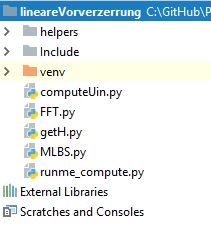
\includegraphics[scale=0.5 ]{slides/Gegeben/lineareFiles.JPG} 
	\end{textblock}	
	\begin{textblock}{20}(93,55)
    	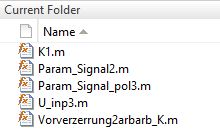
\includegraphics[scale=0.5 ]{slides/Gegeben/matlabFiles.JPG} 
	\end{textblock}	
}

}
\end{frame}


\begin{frame}
\frametitle{Code: Vorgehensweise}

\only<2->{
\begin{itemize}
	\only<1->{\item Refactoring / Anpassung der Matlab-Funktionen an unser Design}
	\only<3->{\item Portierung der Matlab-Funktionen nach Python}
	\only<4->{\item Überprüfung der portierten Funktionen mithilfe von \textbf{TDD}}
	\only<5->	
	{
		\begin{itemize}
			\item  Momentan jeweils 10 korrespondierende \textbf{Unit Tests} in Matlab und Python
		\end{itemize}
	}
	\only<6->{\item Maximale Vorbereitung der Funktionen ohne Messaufbau dank \textbf{TDD}}
	\only<7->
	{
		\begin{itemize}
			\item  Nur zum Testen von \texttt{measure\_Uout} sind Geräte notwendig
		\end{itemize}
	}		
\end{itemize}
}
 

\end{frame}


\section{Erreichtes}

\subsection{Gerätekommunikation}
\begin{frame}{Dokumentation und Gerätekommunikation  }

\begin{itemize}
	
	\item Dokumentation \uncover<2-> {: 
		\begin{itemize}
			\item Handhabung der Geräte, Vorgehensweise bei Tests
			\item Bedienung des Programms 
			\item Ausführliches Kommentieren der Code-Funktionalität
		\end{itemize}
		}
	\item Gerätekommunikation \uncover<3-> {:
		\begin{itemize}
			\item Treiber und Programmer-Manuals zur Nutzung des Programms von anderen Geräten aus 
			\item Laufzeitoptimierung durch Abfrage von Gerätezuständen mittels VISA
			\item Verbesserung der Auflösung des Signals durch Anpassung der Darstellung des Oszilloskops mittels VISA
		\end{itemize}
		}
	
	
\end{itemize}

\end{frame}





\subsection{Code}


\begin{frame}[fragile]
\ifnum\WertA=1
\frametitle{Code: Das Design}
\else
\frametitle{Code: Evaluierung}
\fi

%\only<1>
%	{ 
%\framebox{   %   % just so you can see where the "picture" is

\setcounter{onlyAt}{0}

\ifnum\WertA=1

%\setcounter{onlyAt}{\value{onlyAt}+1}
%\only<\value{onlyAt}>
%{
%	\begin{center}
%		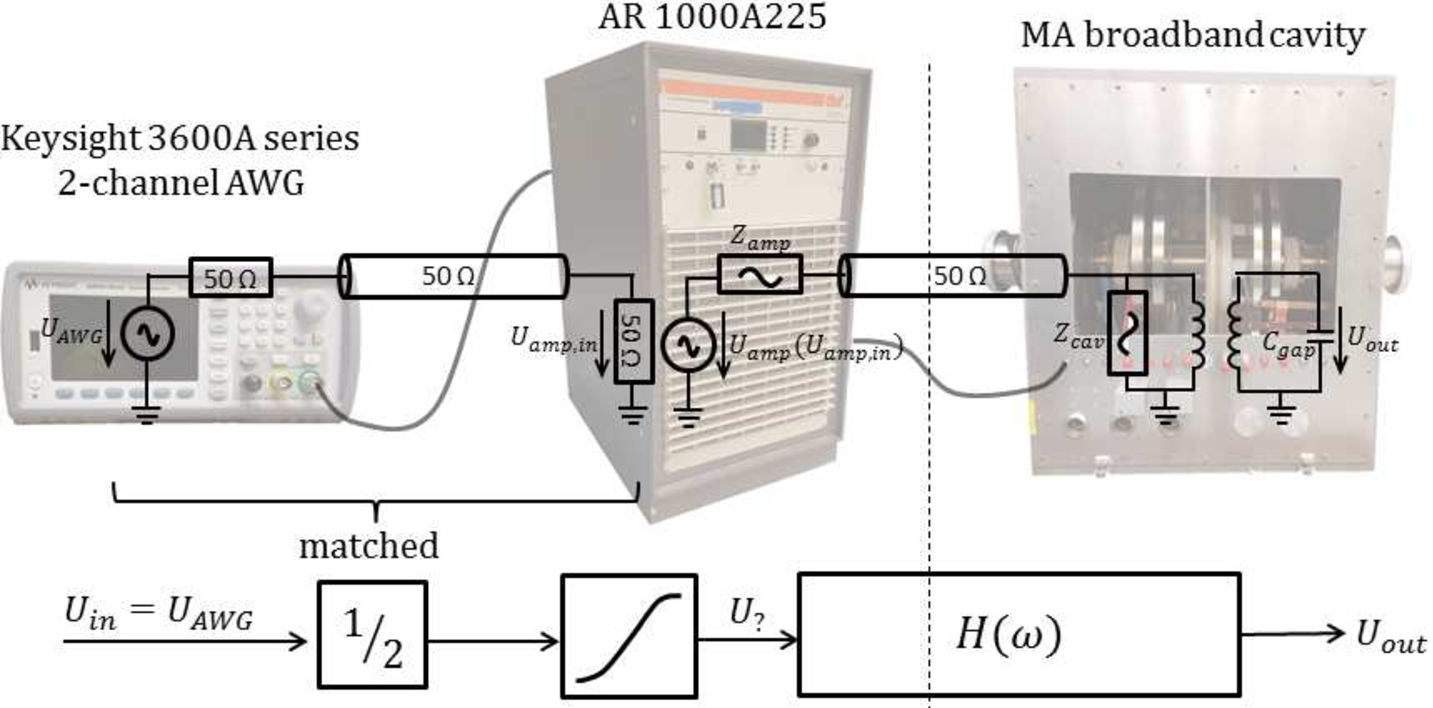
\includegraphics[scale=0.45]{slides/ResultCode/WEPVA047f2_2-eps-converted-to.pdf} 
%	\end{center}
%}

\setcounter{onlyAt}{\value{onlyAt}+1}
\only<\value{onlyAt}>
	{
	\begin{picture}(100,70)
		\put(15,0){
			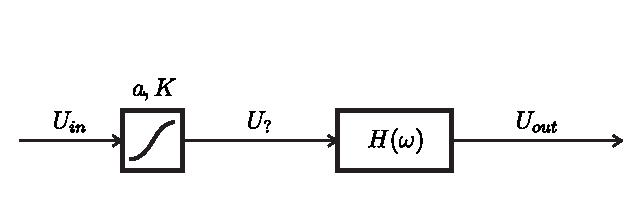
\includegraphics[scale=1.0]{slides/ResultCode/Slide1.eps} 
		}  
	\end{picture} 
	}
\fi
		
\setcounter{onlyAt}{\value{onlyAt}+1}
\only<\value{onlyAt}>
	{
	\begin{picture}(100,70)
		\put(15,0){
			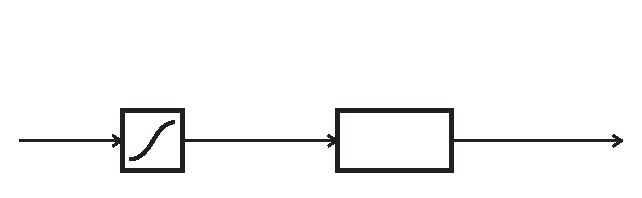
\includegraphics[scale=1.0]{slides/ResultCode/Slide2.eps} 
		}  
	\end{picture} 
	}
	


\ifnum\WertA=1 \setcounter{from}{\value{onlyAt}+1} \setcounter{till}{\value{onlyAt}+1} \else \setcounter{from}{\value{onlyAt}+1} \setcounter{till}{\value{onlyAt}+2} \fi	
\only<\value{from} - \value{till}> 
	{
	\begin{picture}(100,70)
		\put(15,0){
			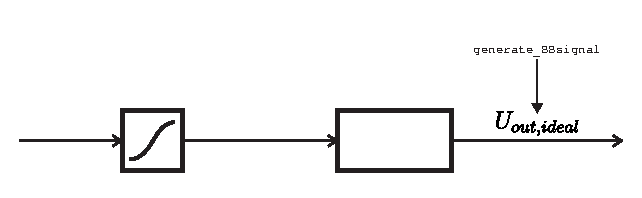
\includegraphics[scale=1.0]{slides/ResultCode/Slide3.eps} 
		}  
	\end{picture} 
	\lstinputlisting[firstline=1,lastline=1]{slides/ResultCode/file.txt} 
	}	
	
\ifnum\WertA=2
	\setcounter{onlyAt}{\value{from} + 1}
	\only<\value{onlyAt}>
	{
		\begin{textblock}{20}(80,50)
    		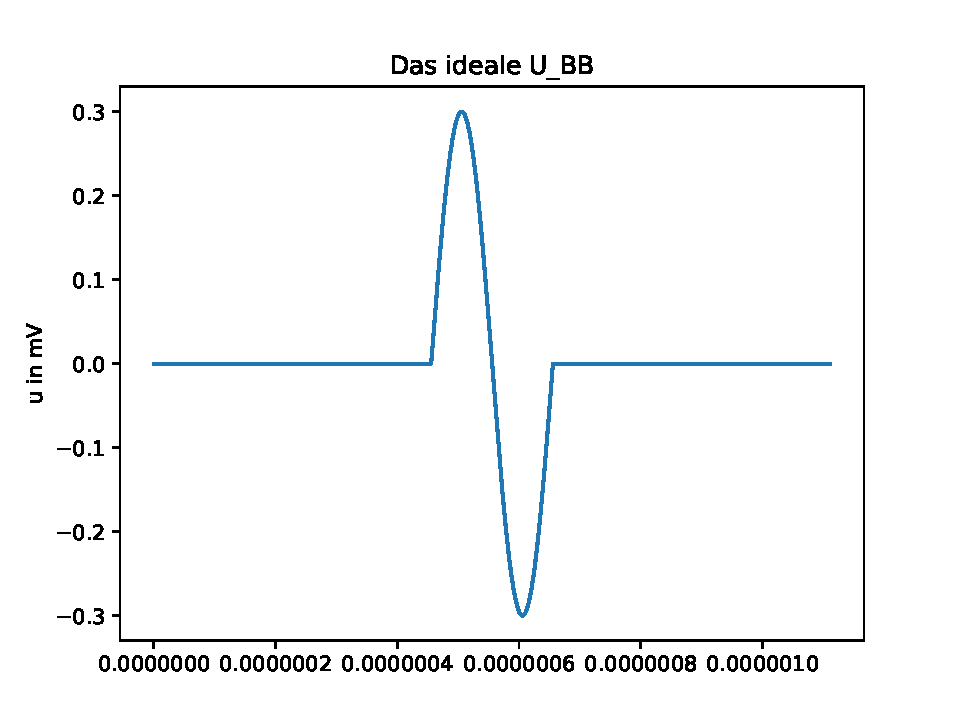
\includegraphics[height=3.5cm, width=4.5cm ]{slides/ResultCode/plots/Uout_ideal.pdf} 
		\end{textblock}	
	} 	
\fi	
\setcounter{onlyAt}{\value{till}}


\ifnum\WertA=1 \setcounter{from}{\value{onlyAt}+1} \setcounter{till}{\value{onlyAt}+1} \else \setcounter{from}{\value{onlyAt}+1} \setcounter{till}{\value{onlyAt}+2} \fi	
\only<\value{from} - \value{till}> 
	{
	\begin{picture}(100,70)
		\put(15,0){
			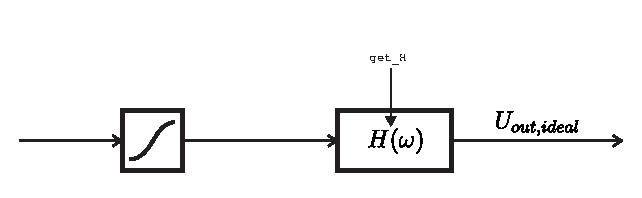
\includegraphics[scale=1.0]{slides/ResultCode/Slide4.eps} 
		}  
	\end{picture} 
	\lstinputlisting[firstline=1,lastline=2]{slides/ResultCode/file.txt} 
	}
	
\ifnum\WertA=2
	\setcounter{onlyAt}{\value{from} + 1}
	\only<\value{onlyAt}>
	{
		\begin{textblock}{20}(93,50)
    		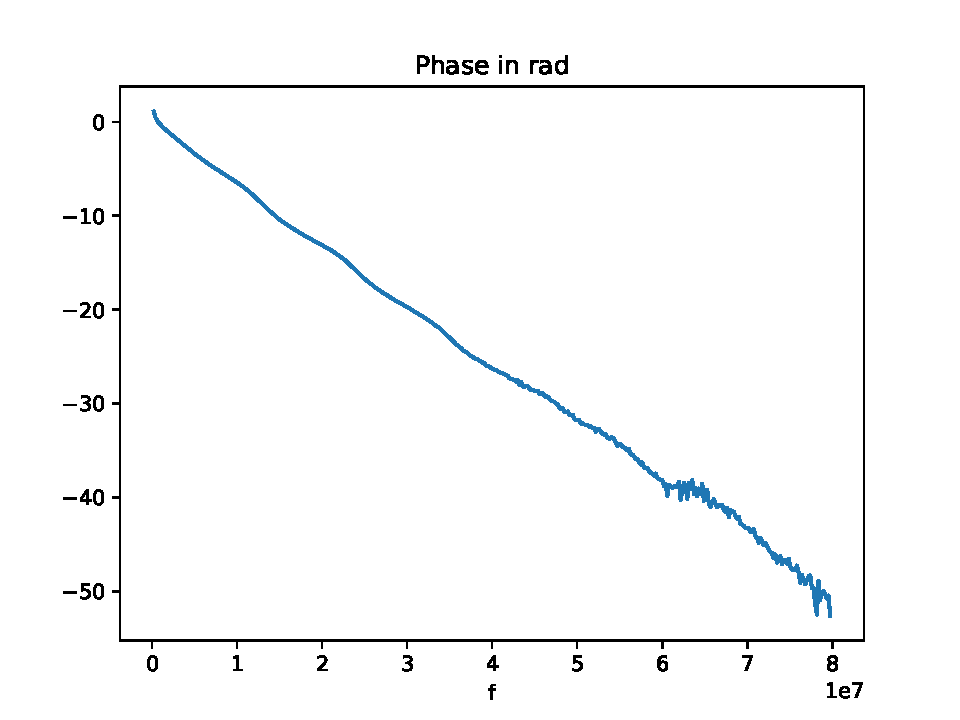
\includegraphics[ width=3.5cm, height=3.1cm ]{slides/ResultCode/plots/H_p.pdf} 
		\end{textblock}			
		\begin{textblock}{20}(61,50)
    		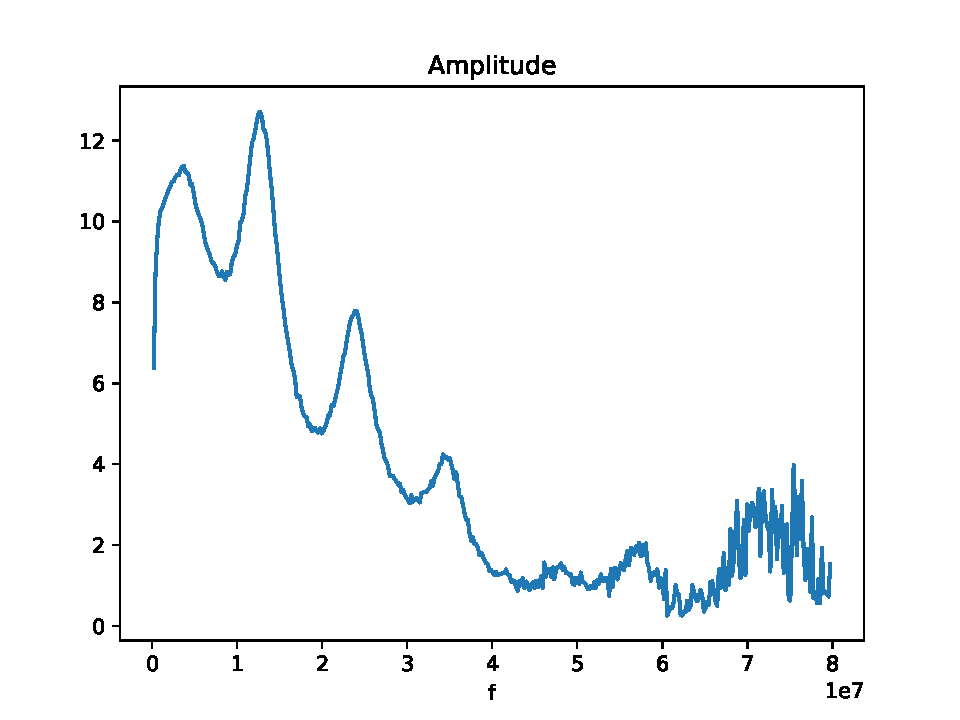
\includegraphics[ width=3.5cm, height=3.1cm]{slides/ResultCode/plots/H_a.pdf} 
		\end{textblock}	
		
	} 	 
\fi	
\setcounter{onlyAt}{\value{till}} 

\setcounter{onlyAt}{\value{onlyAt}+1}
\only<\value{onlyAt}>
	{
	\begin{picture}(100,70)
		\put(15,0){
			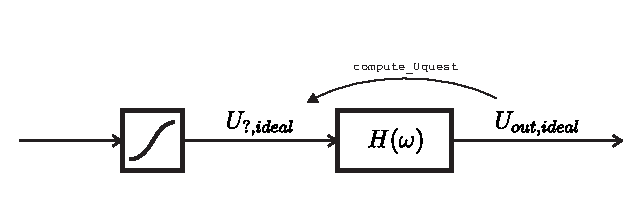
\includegraphics[scale=1.0]{slides/ResultCode/Slide5.eps} 
		}  
	\end{picture} 
	\lstinputlisting[firstline=1,lastline=3]{slides/ResultCode/file.txt} 
	}	
	
\setcounter{onlyAt}{\value{onlyAt}+1}
\only<\value{onlyAt}>
	{
	\begin{picture}(100,70)
		\put(15,0){
			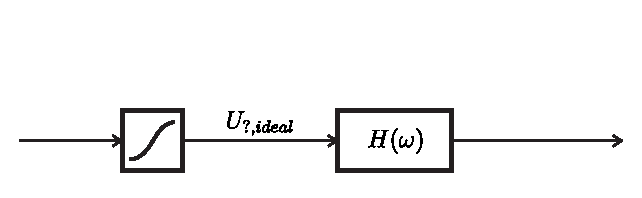
\includegraphics[scale=1.0]{slides/ResultCode/Slide5-1.eps} 
		}  
	\end{picture} 
	\lstinputlisting[firstline=1,lastline=3]{slides/ResultCode/file.txt} 
	}
	
\ifnum\WertA=2
	\setcounter{from}{\value{onlyAt}} 
	\setcounter{till}{\value{onlyAt}+2}
	\only<\value{from} - \value{till}>
	{
		\begin{textblock}{20}(80,50)
    		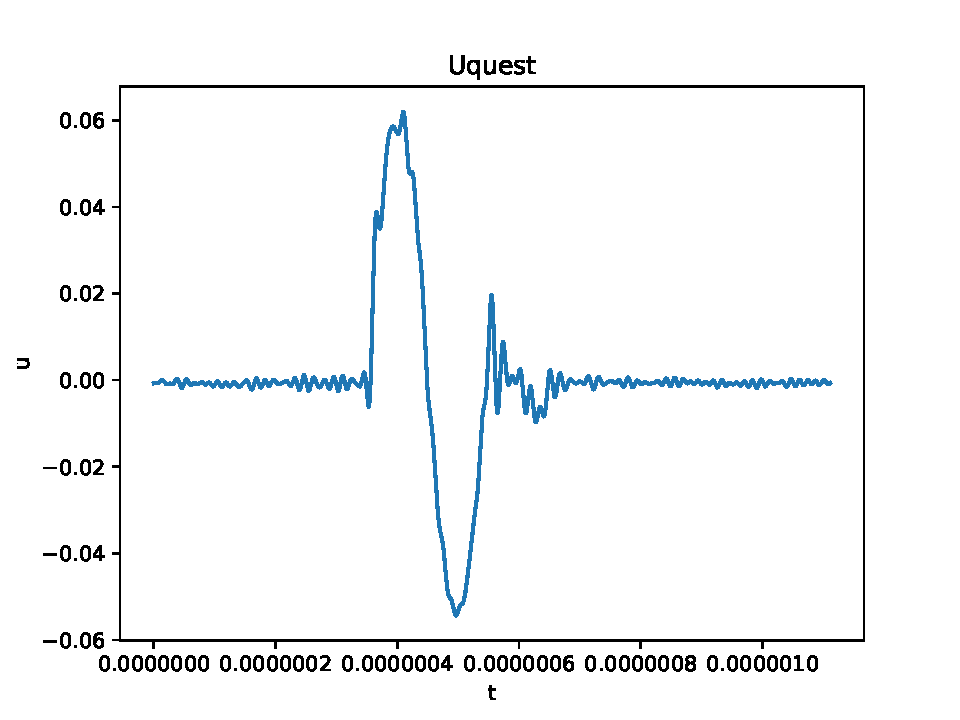
\includegraphics[height=3.5cm, width=4.5cm ]{slides/ResultCode/plots/U_quest_ideal.pdf} 
		\end{textblock}	
	} 
\fi	

\setcounter{onlyAt}{\value{onlyAt}+1}
\only<\value{onlyAt}>
{
	\begin{picture}(100,70)
		\put(15,0)
		{
			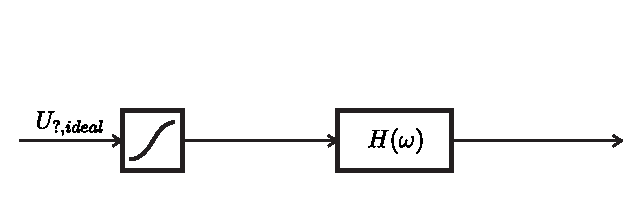
\includegraphics[scale=1.0]{slides/ResultCode/Slide6.eps} 
		}  
	\end{picture} 
	\lstinputlisting[firstline=1,lastline=3]{slides/ResultCode/file.txt} 
}

\setcounter{onlyAt}{\value{onlyAt}+1}
\only<\value{onlyAt}>
{
	\begin{picture}(100,70)
		\put(15,0)
		{
			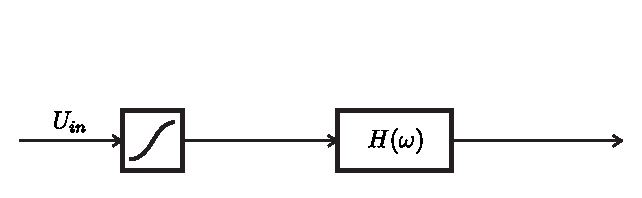
\includegraphics[scale=1.0]{slides/ResultCode/Slide7.eps} 
		}
	\end{picture} 	
	\lstinputlisting[firstline=1,lastline=4]{slides/ResultCode/file.txt} 	
}	

\setcounter{onlyAt}{\value{onlyAt}+1}
\only<\value{onlyAt}>
{
	\begin{picture}(100,70)
		\put(15,0)
		{
			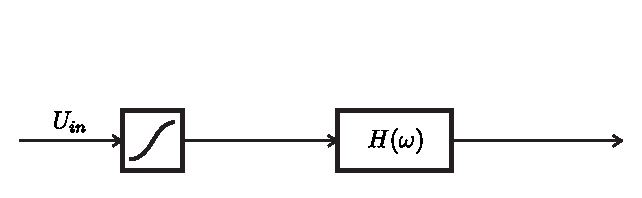
\includegraphics[scale=1.0]{slides/ResultCode/Slide7.eps} 
		}
	\end{picture} 	
	\lstinputlisting[firstline=1,lastline=5]{slides/ResultCode/file.txt} 		

}

\ifnum\WertA=1 \setcounter{from}{\value{onlyAt}+1} \setcounter{till}{\value{onlyAt}+1} \else \setcounter{from}{\value{onlyAt}+1} \setcounter{till}{\value{onlyAt}+3} \fi	
\only<\value{from} - \value{till}> 
{
	\begin{picture}(100,70)
		\put(15,0)
		{
			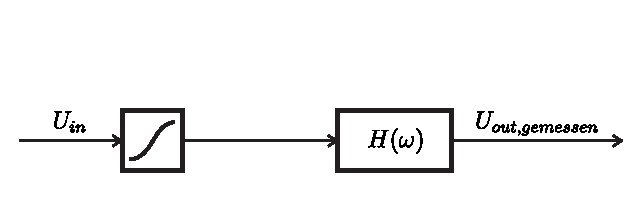
\includegraphics[scale=1.0]{slides/ResultCode/Slide8.eps} 
		}
	\end{picture} 	
	\lstinputlisting[firstline=1,lastline=5]{slides/ResultCode/file.txt} 		

}

\ifnum\WertA=2
	\setcounter{onlyAt}{\value{from}+1}
	\only<\value{onlyAt}>
	{
		\begin{textblock}{20}(80,50)
    		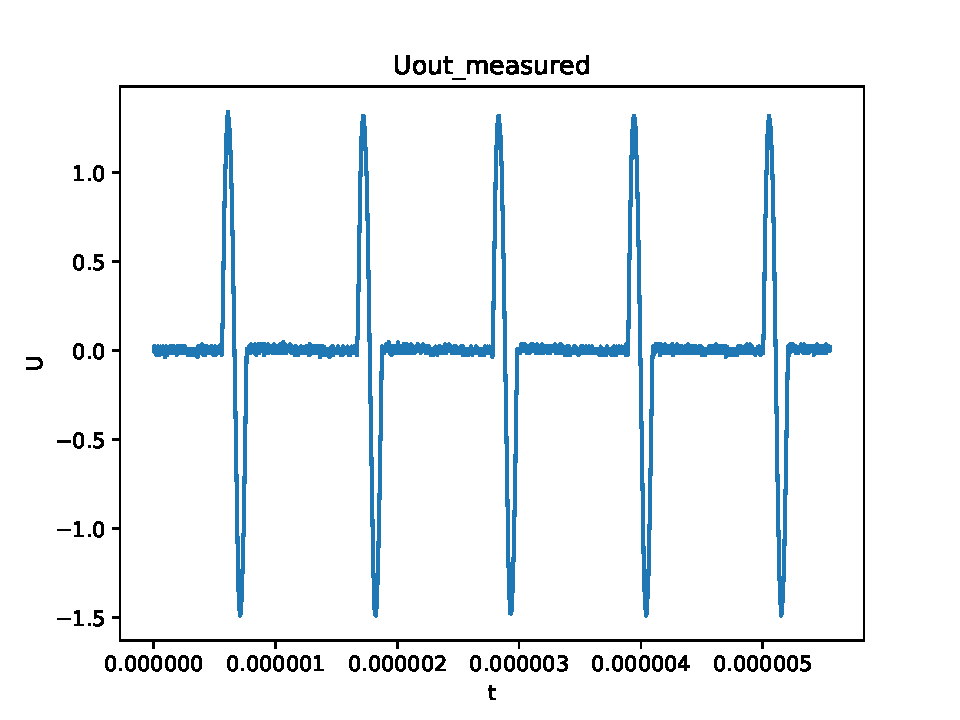
\includegraphics[height=3.5cm, width=4.5cm ]{slides/ResultCode/plots/Uout_measured.pdf} 
		\end{textblock}	
	} 
	\setcounter{onlyAt}{\value{from}+2}
	\only<\value{onlyAt}>
	{
		\begin{textblock}{20}(80,50)
    		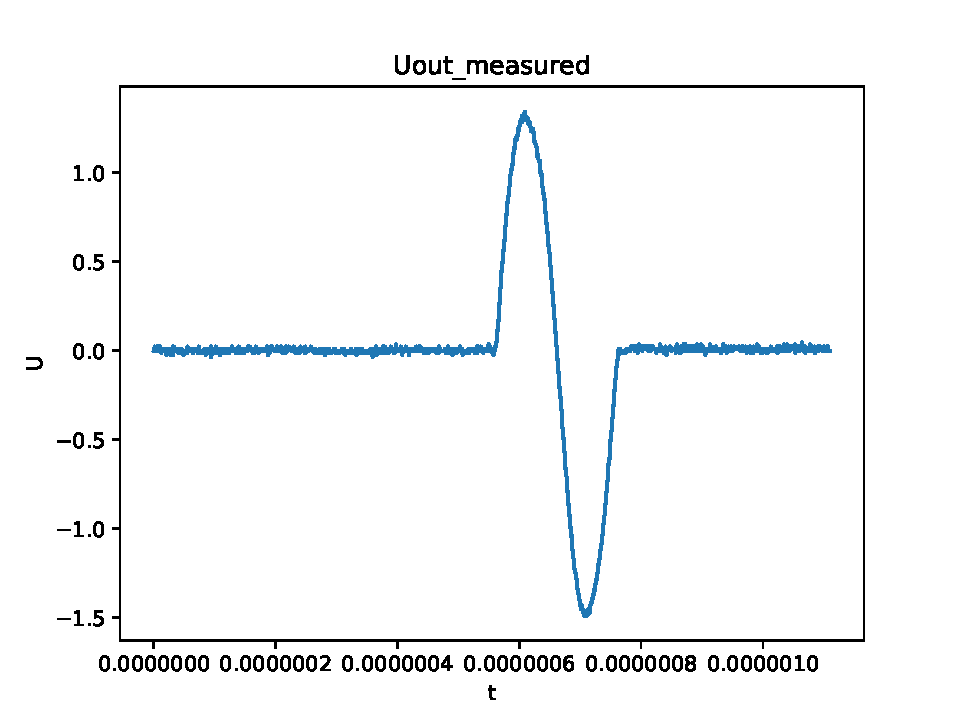
\includegraphics[height=3.5cm, width=4.5cm ]{slides/ResultCode/plots/Uout_measured_cut.pdf} 
		\end{textblock}	
	} 
\fi
\setcounter{onlyAt}{\value{till}} 
 
\ifnum\WertA=1 \setcounter{from}{\value{onlyAt}+1} \setcounter{till}{\value{onlyAt}+1} \else \setcounter{from}{\value{onlyAt}+1} \setcounter{till}{\value{onlyAt}+2} \fi	
\only<\value{from} - \value{till}> 
{
	\begin{picture}(100,70)
		\put(15,0)
		{
			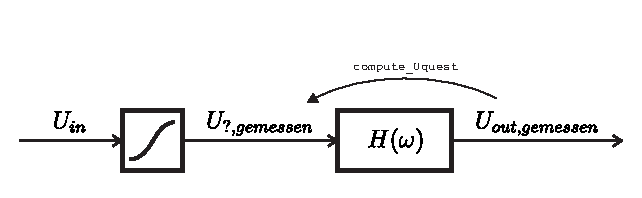
\includegraphics[scale=1.0]{slides/ResultCode/Slide9.eps} 
		}  
	\end{picture} 
	\lstinputlisting[firstline=1,lastline=6]{slides/ResultCode/file.txt} 
}	

\ifnum\WertA=2
	\setcounter{onlyAt}{\value{from} + 1}
	\only<\value{onlyAt}>
	{
		\begin{textblock}{20}(80,50)
    		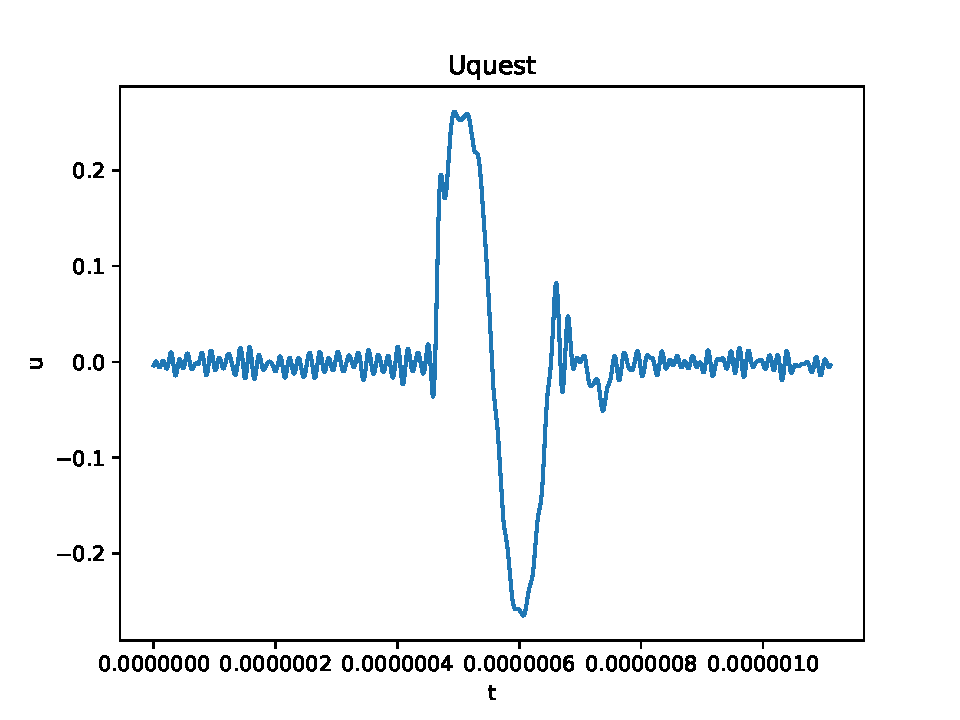
\includegraphics[height=3.5cm, width=4.5cm ]{slides/ResultCode/plots/U_quest_measured.pdf} 
		\end{textblock}	
	}
\fi
\setcounter{onlyAt}{\value{till}} 
	
\ifnum\WertA=1 \setcounter{from}{\value{onlyAt}+1} \setcounter{till}{\value{onlyAt}+1} \else \setcounter{from}{\value{onlyAt}+1} \setcounter{till}{\value{onlyAt}+2} \fi	
\only<\value{from} - \value{till}> 
{
	\begin{picture}(100,70)
		\put(15,0){
			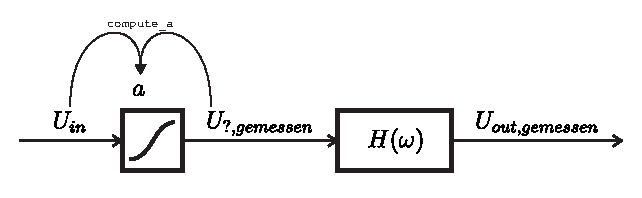
\includegraphics[scale=1.0]{slides/ResultCode/Slide10.eps} 
		}  
	\end{picture} 
	\lstinputlisting[firstline=1,lastline=7]{slides/ResultCode/file.txt} 
}

\ifnum\WertA=2
	\setcounter{onlyAt}{\value{from} + 1}
	\only<\value{onlyAt}>
	{
		\begin{textblock}{20}(65,72)
    		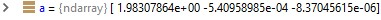
\includegraphics[scale=0.6 ]{slides/ResultCode/plots/a.JPG} 
		\end{textblock}	
	} 
\fi	
\setcounter{onlyAt}{\value{till}}	


\ifnum\WertA=1 \setcounter{from}{\value{onlyAt}+1} \setcounter{till}{\value{onlyAt}+1} \else \setcounter{from}{\value{onlyAt}+1} \setcounter{till}{\value{onlyAt}+2} \fi	
\only<\value{from} - \value{till}> 
{
	\begin{picture}(100,70)
		\put(15,0)
		{
			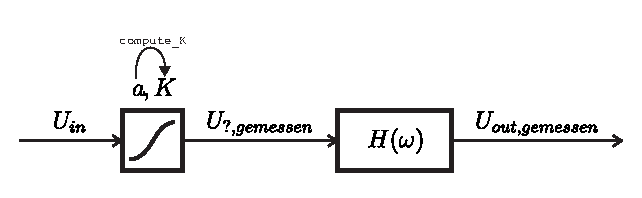
\includegraphics[scale=1.0]{slides/ResultCode/Slide11.eps} 
		}  
	\end{picture} 
	\lstinputlisting[firstline=1,lastline=8]{slides/ResultCode/file.txt} 
}

\ifnum\WertA=2
	\setcounter{onlyAt}{\value{from} + 1}
	\only<\value{onlyAt}>
	{
		\begin{textblock}{20}(80,50)
    		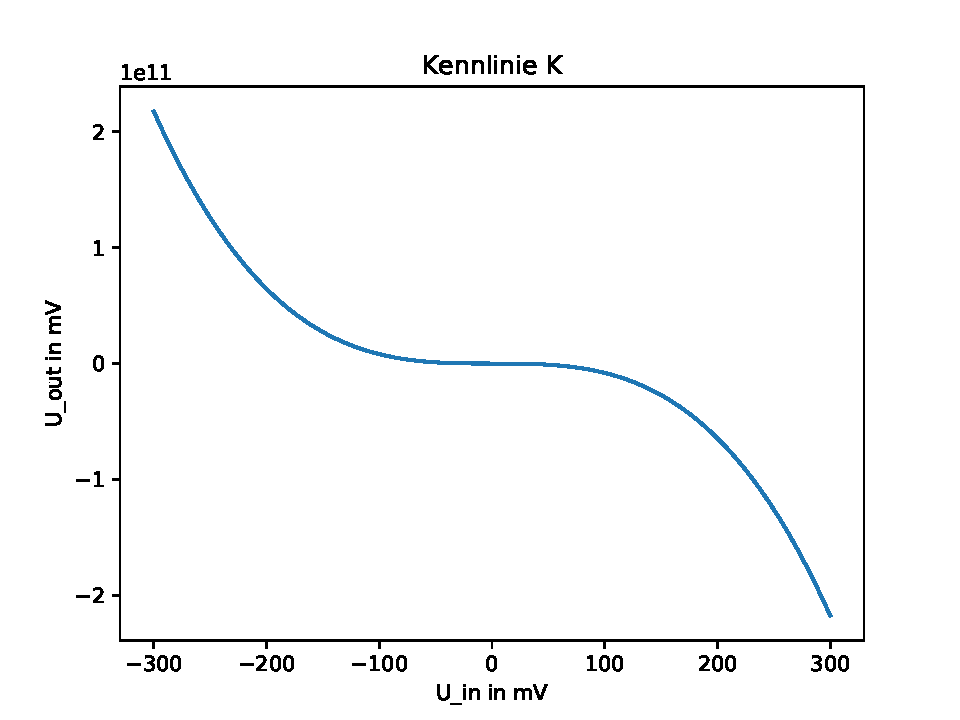
\includegraphics[height=3.5cm, width=4.5cm ]{slides/ResultCode/plots/K.pdf} 
		\end{textblock}	
	} 
\fi	
\setcounter{onlyAt}{\value{till}}	

\setcounter{onlyAt}{\value{onlyAt}+1}
\only<\value{onlyAt}>
{
	\begin{picture}(100,70)
		\put(15,0)
		{
			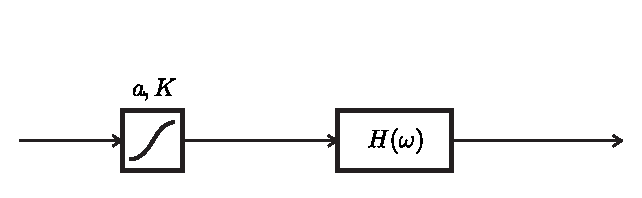
\includegraphics[scale=1.0]{slides/ResultCode/Slide12-0.eps} 
		}  
	\end{picture} 
	\lstinputlisting[firstline=1,lastline=8]{slides/ResultCode/file.txt} 
}
	
\setcounter{onlyAt}{\value{onlyAt}+1}
\only<\value{onlyAt}>
{
	\begin{picture}(100,70)
		\put(15,0)
		{
			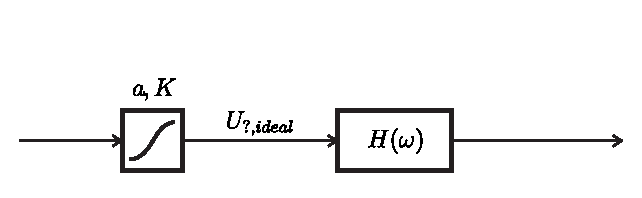
\includegraphics[scale=1.0]{slides/ResultCode/Slide12-01.eps} 
		}  
	\end{picture} 
	\lstinputlisting[firstline=1,lastline=8]{slides/ResultCode/file.txt} 
}
	
\ifnum\WertA=1 \setcounter{from}{\value{onlyAt}+1} \setcounter{till}{\value{onlyAt}+1} \else \setcounter{from}{\value{onlyAt}+1} \setcounter{till}{\value{onlyAt}+2} \fi	
\only<\value{from} - \value{till}> 
{
	\begin{picture}(100,70)
		\put(15,0)
		{
			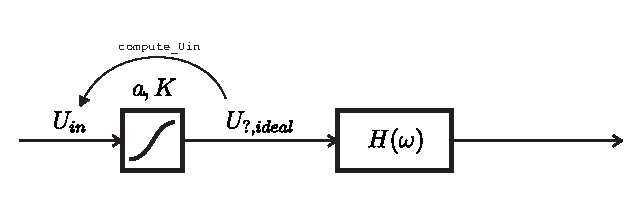
\includegraphics[scale=1.0]{slides/ResultCode/Slide12.eps} 
		}  
	\end{picture} 
	\lstinputlisting[firstline=1,lastline=9]{slides/ResultCode/file.txt} 
}

\ifnum\WertA=2
	\setcounter{onlyAt}{\value{from} + 1}
	\only<\value{onlyAt}>
	{
		\begin{textblock}{20}(80,50)
    		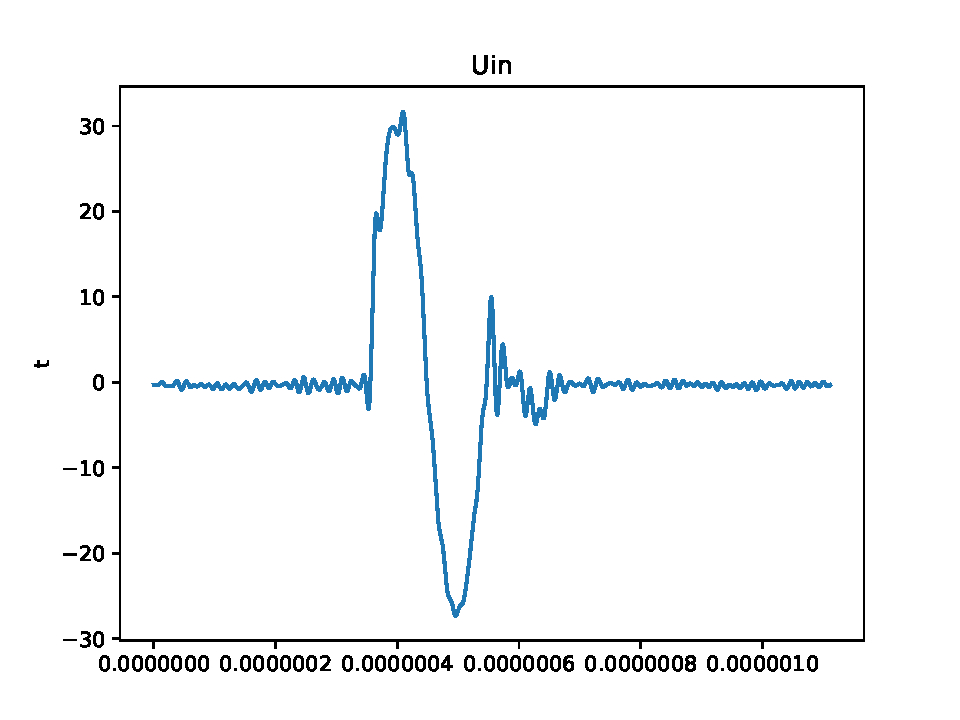
\includegraphics[height=3.5cm, width=4.5cm ]{slides/ResultCode/plots/U_in.pdf} 
		\end{textblock}	
	} 
\fi	
\setcounter{onlyAt}{\value{till}}
	
\setcounter{onlyAt}{\value{onlyAt}+1}
\only<\value{onlyAt}>
{
	\begin{picture}(100,70)
		\put(15,0)
		{
			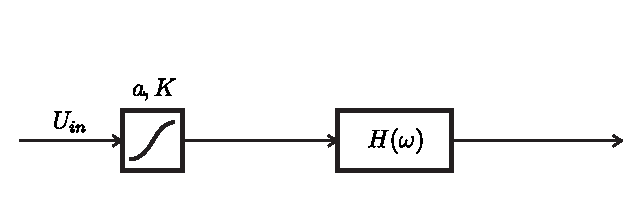
\includegraphics[scale=1.0]{slides/ResultCode/Slide13-0.eps} 
		}  
	\end{picture} 
	\lstinputlisting[firstline=1,lastline=9]{slides/ResultCode/file.txt} 
}



%\setcounter{onlyAt}{\value{onlyAt}+1}
%\only<\value{onlyAt}>
%{
%	\begin{picture}(100,70)
%		\put(15,0)
%		{
%			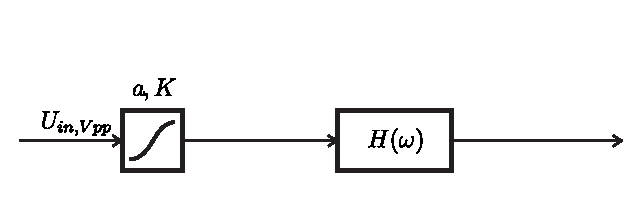
\includegraphics[scale=1.0]{slides/ResultCode/Slide13-01.eps} 
%		}  
%	\end{picture} 
%	\lstinputlisting[firstline=1,lastline=10]{slides/ResultCode/file.txt} 
%}
	
\setcounter{onlyAt}{\value{onlyAt}+1}
\only<\value{onlyAt}>
{
	\begin{picture}(100,70)
		\put(15,0)
		{
			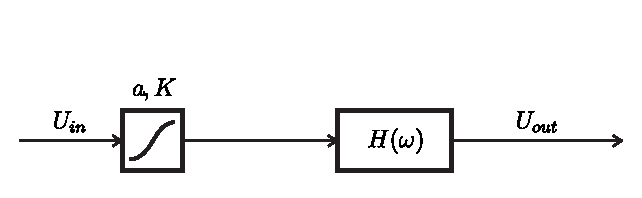
\includegraphics[scale=1.0]{slides/ResultCode/Slide13.eps} 
		}  
	\end{picture} 
	\lstinputlisting[firstline=1,lastline=10]{slides/ResultCode/file.txt} 
}

  
%	\begin{figure}[t]
%	
%%	
%	\end{figure}	
	%}
%\only<2>{ \lstinputlisting[firstline=1,lastline=2]{slides/ResultCode/file.txt} }
%\only<3>{ \lstinputlisting[firstline=1,lastline=3]{slides/ResultCode/file.txt} }
%\only<4>{ \lstinputlisting[firstline=1,lastline=4]{slides/ResultCode/file.txt} }
%\only<5>{ \lstinputlisting[firstline=1,lastline=5]{slides/ResultCode/file.txt} }
%\only<6>{ \lstinputlisting[firstline=1,lastline=6]{slides/ResultCode/file.txt} }
%\only<7>{ \lstinputlisting[firstline=1,lastline=7]{slides/ResultCode/file.txt} }
%\only<8>{ \lstinputlisting[firstline=1,lastline=8]{slides/ResultCode/file.txt} }
%\only<9>{ \lstinputlisting[firstline=1,lastline=9]{slides/ResultCode/file.txt} }
%\only<10>{ \lstinputlisting[firstline=1,lastline=10]{slides/ResultCode/file.txt} }


\end{frame}





\section{Evaluierung}
\subsection{Gerätekommunikation}
\begin{frame}{Evaluierung: Dokumentation und Gerätekommunikation}

%Stand letzter Test
Unvollständige Dokumentation:
\begin{itemize}
	\item Ausführliche Beschreibung von In- und Output-Formaten von Methoden
	\item Begründung von nicht-trivialen Umformungsschritten in Methoden
\end{itemize}

Getestet und funktionsfähige Aspekte der Gerätekommunikation:
\begin{itemize}
	\item VISA-Protokoll und PyVisa Package Installation 
	\item Kommunikation mit AWG von anderem Laptop aus über USB
\end{itemize}

Noch nicht erfolgreich getestete Aspekte der Gerätekommunikation:
\begin{itemize}
	\item Kommunikation mit Oszilloskop von anderem Laptop aus über LAN
	\item Laufzeit: Status-Abfrage der Geräte mit \lstinline{BUSY?} oder \lstinline{*WAI}
	\item Anpassung der Auflösung [\textit{noch nicht implementiert}]
\end{itemize}

\end{frame}





\subsection{Code}
\begin{frame}{Evaluierung: Python-Code für die nichtlinere Verzerrung}

\end{frame}





\section{Ausblick}
\documentclass[../Report.tex]{subfiles}


\begin{document}


\chapter{Ausblick}
\label{chap:ausb}
---- In diesem Kapitel wird auf offene Fragen / neue Probleme / Anstöße für weitere Arbeiten eingegangen. Dabei sollte es um eher inhaltliche Aspekte gehen (u. U. wenig to dos für Code-Design) gegebenenfalls darf hier bei vielem auf die Erfahrungen aus den vorigen Kapiteln verwiesen werden und damit einen Übersichts-Charakter haben (erleichtert nachfolgenden Projekten die Arbeit) --- 

\section{Impressionen zum Code}
\label{sec:ausb.code}
In Bezug auf das Design des Codes verbleiben eine Reihe Anregungen und Gedanken, die nicht realisiert wurden, je nach Ausführung aber interessant zu bedenken sein könnten.

\begin{itemize}
	\item	Die Geräte AWG und DSO als Klassen einzubinden könnte den Vorteil bieten, alle SCPI Commands an einer Stelle zu bündeln und den Zugriff darauf allgemeingültig zu halten.
	
	\item	Eine Einbindung des momentanen Programms in die RF-Tools des GSI-Standards könnte in zwei Teilen erfolgen. Die bestehende Funktionalität zur Berechnung von $K$ und $\Hcompl$ kann unabhängig der Optimierungsalgorithmen genutzt werden. Dabei ist insbesondere zu prüfen, ob oder wie die Aspekte im \nameref{chap:code} beibehalten werden. 
	
	\item 	Die momentane Version ist in erster Linie über eine Python-IDE ausführbar. Die Ausführung über die Kommandozeile wurde nicht fokussiert.
	\item Für die Erstellung eines idealen Barrier-Bucket Ausgangssignals wird momentan noch eine selbst implementierte Methode verwendet. Dafür kann auch das vorhandene RF-Tool verwendet werden.
	
\end{itemize}





\section{Ausblick: Optimierung}
\label{sec:ausb.opti}

- (offene Punkte K-Optimierung?)


Auf den Ergebnissen aus \nameref{chap:opt} aufbauend, verbleiben eine Reihe von offenen Fragestellungen:

\begin{enumerate}
	\item 	Wie wirkt sich die Optimierung von $K$ aufgrund ihrer Nichtlinearität auf die Übertragungsfunktion $\Hcompl$ aus und muss dies in der Optimierung berücksichtigt werden, etwa in der Reihenfolge der Iterationsschritte?
	
	\item	Wie wird mit der Tatsache umgegangen, dass im Frequenzbereich unabhängig der Qualität der Messung nur etwa halb so viele Daten für die Anpassung zur Verfügung stehen, wie in $\Hcompl$ selbst vorliegen?
	
	\item 	Ist die getrennte Interpolation von Betrag und Phase der Signalspektren auf die Frequenzen der Übertragungsfunktion in der Optimierung von $\Hcompl$ die beste Lösung? 
	
	\item	In welcher Reihenfolge wird die Iteration durchgeführt? Wird zuerst $\Hcompl$ in mehreren Durchgängen angepasst und danach $K$? Oder im Wechsel je eine Iteration?
	
	\item 	Wie wird die Auswahl der Schrittweiten $\sigma_H$ und $\sigma_a$ vorgenommen? Werden diese pauschal einmal festgesetzt zu Beginn des Algorithmus oder ist eine dynamische Anpassung, etwa durch die Qualität des letzten gemessenen Signals oder in Abhängigkeit des Iterationsschritts vorzuziehen? 
	
	\item 	Wie lässt sich der Einfluss von zufälligem Rauschen auf die Optimierung reduzieren? Insbesondere die Auflösung im höherfrequenten Betragsspektrum ist hier problematisch. Und im Falle des Ignorieren von Korrekturen an als fehlerhaft befundenen Frequenzen: Auf welchen Wert wird der Korrekturterm bei diesen Frequenzen gesetzt?
	
	\item	Wie lassen sich die im idealen Spektrum des Einzelsinus enthaltenen Nulldurchgänge in der Optimierung von $\Hcompl$ berücksichtigen, um interpolationsbedingt große Fehlerterme zu vermeiden? Ist das einfache Ignorieren dieser Frequenzen für die Anpassung eine Möglichkeit? Und in welchem kleinen Frequenzbereich um einen Nulldurchgang müssten dann die Werte ignoriert werden?
	
	\item 	Wie - insofern überhaupt - ist eine Optimierung der Phase von $\Hcompl$ zu gestalten?
	
	\item	Nach welchem Qualitätsmerkmal wird das Signal bewertet und wie wirkt sich dies auf den Algorithmus aus?
	
	\item	Gibt es eine sinnvolle Abbruchbedingung, mit der die Iteration versehen werden sollte? Etwa, dass sich die Qualität im Vergleich zu den vorherigen Iterationen nicht mehr mit ähnlicher Rate verbessert hat? Der Trade-Off liegt zwischen Laufzeit und Signal-Qualität.
	
	\item	Wie bestimmt man die Grenzen, in denen $K$ genutzt werden kann? Wie kann man garantieren, dass $K$ in den Bereichen, aus denen die Daten zur Berechnung von $a_n$ benutzten werden, bijektiv ist?
	
	\item	Gibt es eine Möglichkeit die Grenzen von $K$ bei der Optimierung zu erweitern? Ein möglicher Indikator: Kann man die Rückgabe von \lstinline{numpy.linalg.lstsq(LGS)} aus der Berechnung von $a_n$ nutzen, um eine Aussage über die Abweichung der Werte zu treffen?
\end{enumerate}





\section{--- Gerätekomm---}
\label{sec:ausb.geraete}
--- in dieser Section werden weitere Punkte der Geräte-Komm aufgegriffen, etwa - die (geringe) Auflösung des AWG im Kontext der Optimierung (ggf. in \ref{sec:ausb.opti} besser?) , die Einbindung des neuen Oszis oder die Idee der Klassen-Implementierung 
%TODO: prüfe Redundanz mit Abschnitt Gerätekommunikation! nur eine Einbindung, wo ist sie sinnvoller? 

%TODO: Überlegung ausführen, ob RF-Tools einbinden hier sinnvoller ist als in "Offenen Fragen" im Abschnitt Code-Design?






\end{document}

	
%\section{Motivation}
%\begin{frame}
%\frametitle{Motivation}
%	\begin{itemize}
%	\item field/circuit coupling enables detailed simulation of the electromagnetic field inside a device coupled to a circuit
%	
%	\item can be achieved using a Waveform Relaxation (WR) scheme
%	
%	\item used to simulate the protection system of the superconducting magnets at the LHC (CERN)
%	\end{itemize}
%\end{frame}
%
%\begin{frame}
%\frametitle{Problem setting}
%	\begin{itemize}
%	\item solving the equations formulated during field/circuit coupling monolithically is computationally costly 
%	
%	\item WR can provide speed up by applying different solvers for field and circuit parts respectively
%	
%	\item parallelising parts of the simulation could provide further speed up \linebreak $\rightarrow$ Parareal is a parallel in time integration method
%	
%	\item How can WR and Parareal be combined efficiently?
%	\end{itemize}
%\end{frame}
%		
%%%%%%%%%%%%%%%%%%%%%%%%%%%%%%%%%%%%%%%%%%%%%%%%%%%%%%%%%%%%%%%%%%%%%%%%%%%%%%%%%%%%%%%%%%%%%%%%%%%%%%%%%%%%%%%%%%%%%%%%%%%%%%%%%%%%%%%
%
%\section{Problem setting}
%\begin{frame}
%\frametitle{Magnetic Vector Potential (MVP)}
%	\begin{itemize}
%	\item in the continous form the MVP is denoted as $\vec{A}$ and the equation reads
%	\begin{equation*}
%	\nabla\times(\nu\nabla\times\vec{A}) + \sigma\frac{\partial\vec{A}}{\partial \mathit{t}} = \vec{J}_{\mathrm{src}}
%	\end{equation*}
%	where $\nu$ = $\mu^{-1}$ is the reluctivity, $\mu>0$ the permeability and $\sigma\geq0$ the conductivity
%	
%	\item MVP and current through the MQS device are coupled by \textit{winding functions} denoted as $\vec{\chi}$
%	\begin{equation*}
%\vec{J}_{\mathrm{src}} = \vec{\chi}\ \mathbf{i}
%	\end{equation*}
%	where $\vec{J}_{\mathrm{src}}$ is the current density inside the MQS device and $\mathbf{i}$ the current in the circuit	
%	\end{itemize}
%\end{frame}
%
%\begin{frame}
%\frametitle{Magnetic Vector Potential (MVP)}
%	\begin{itemize}
%	\item in the discretised form the MVP is denoted as $\mathbf{a}$ and described by the discrete curl-curl equation
%	\begin{equation*}
%	\mathbf{M}_{\sigma}\frac{\mathrm{d}}{\mathrm{d}\mathit{t}}\mathbf{a} + \mathbf{K}_{\nu}(\mathbf{a})\mathbf{a} = \mathbf{j}_{\mathrm{str}}
%	\end{equation*}
%	
%	\item where $\mathbf{M}_{\sigma}$ is the conductivity matrix and $\mathbf{K}_{\nu}(\mathbf{a})$ is the nonlinear curl-curl matrix		
%	
%	\item in the case of stranded conductor models the circuit coupling is given by
%	\begin{equation*}
%	\mathbf{j}_{\mathrm{str}} = \mathbf{X}_{\mathrm{str}}\mathbf{i}_{\mathrm{str}}
%	\end{equation*}
%	and
%	\begin{equation*}
%	\mathbf{X}_{\mathrm{str}}^{T}\frac{\mathrm{d}}{\mathrm{d}\mathit{t}}\mathbf{a} = \mathbf{v}_{\mathrm{str}}
%	\end{equation*}
%	where $\mathbf{X}_{\mathrm{str}}$ is the discretised winding function
%	\end{itemize}
%\end{frame}
%
%\begin{frame}
%\frametitle{Modified Nodal Analysis (MNA)}
%	\begin{itemize}
%	\item the classical modified nodal analysis (MNA) gives the following system of equations
%	\begin{align*}
%	\mathbf{A}_{C}\mathbf{C}_{Q}\mathbf{A}_{C}^{T}\frac{\mathrm{d}\mathbf{u}}{\mathrm{d}\mathit{t}} + \mathbf{A}_{R}\mathbf{G}_{R}\mathbf{A}_{R}^{T}\mathbf{u} + \mathbf{A}_{L}\mathbf{i}_{L} + \mathbf{A}_{V}\mathbf{i}_{v} + \mathbf{A}_{M}\mathbf{i}_{M} + \mathbf{A}_{I}\mathbf{i}_{s}(\mathit{t}) = \mathbf{0}\\
%	\mathbf{L}_{\Phi}\frac{\mathrm{d}\mathbf{i}_{L}}{\mathrm{d}\mathit{t}} - \mathbf{A}_{L}^{T}\mathbf{u} = \mathbf{0}\\
%	\mathbf{A}_{V}^{T}\mathbf{u} - \mathbf{v}_{s}(\mathit{t}) = \mathbf{0}\\
%	\mathbf{A}_{M}^{T}\mathbf{u} - \mathbf{v}_{M}(\mathit{t}) = \mathbf{0}
%	\end{align*}
%	where $\mathbf{A}_*$ denotes the respective incidence matrix, $\mathbf{C}_{Q}$, $\mathbf{G}_{R}$ and $\mathbf{L}_{\Phi}$ are diagonal matrices containing the parameter values and $\mathbf{u}$ contains the node potentials
%	\end{itemize}
%\end{frame}
%
%%%%%%%%%%%%%%%%%%%%%%%%%%%%%%%%%%%%%%%%%%%%%%%%%%%%%%%%%%%%%%%%%%%%%%%%%%%%%%%%%%%%%%%%%%%%%%%%%%%%%%%%%%%%%%%%%%%%%%%%%%%%%%%%%%%%%%%
%	
%\section{Waveform Relaxation}
%\begin{frame}
%\frametitle{Waveform Relaxation}	
%	\begin{itemize}
%	\item subsystems can be solved independently
%	
%	\item solutions of each subsystem are exchanged iteratively until convergence 	
%	\end{itemize}
%	
%	\begin{figure}
%	\begin{tikzpicture}[scale = 1.5]
%    \draw[thick,->] (0,1) -- (6,1);
%    \draw (1, 1) -- (1, 1.1) node [above=1pt]{\textcolor{gray}{$T_{1,1}$}};
%    \draw (3, 1) -- (3, 1.1) node [above=1pt]{\textcolor{gray}{$T_{3,1}$}};
%    \draw (5, 1) -- (5, 1.1) node [above=1pt]{\textcolor{gray}{$T_{5,1}$}};
%    \foreach \t in {1,2,...,5}
%    \draw [-stealth, bend angle=45, bend left]  ({\t-1},1) to (\t,1);                        
%    \draw[thick,->] (0,0) -- (6,0);
%    \draw (0.66, 0) -- (0.66, -0.1) node [below=1pt]{\textcolor{gray}{$T_{1,2}$}};
%    \draw (1.33, 0) -- (1.33, -0.1) node [below=1pt]{\textcolor{gray}{$T_{2,2}$}};
%    \draw (2.66, 0) -- (2.66, -0.1) node [below=1pt]{\textcolor{gray}{$T_{4,2}$}};
%    \draw (3.33, 0) -- (3.33, -0.1) node [below=1pt]{\textcolor{gray}{$T_{5,2}$}};
%    \draw (4.66, 0) -- (4.66, -0.1) node [below=1pt]{\textcolor{gray}{$T_{7,2}$}};
%    \draw (5.33, 0) -- (5.33, -0.1) node [below=1pt]{\textcolor{gray}{$T_{8,2}$}};
%    \foreach \t in {0.66,1.33,...,5.66}
%    \draw [-stealth, bend angle=45, bend right]  ({\t-0.66},0) to (\t,0);                       
%    \draw (0, 0) -- (0, 1.2) node [above=1pt]{$t_0$};
%    \draw (2, 0) -- (2, 1.2) node [above=1pt]{$t_1$};
%    \draw (4, 0) -- (4, 1.2) node [above=1pt]{$t_2$};                       
%    \foreach \t in {2,4}
%    \draw [-stealth, dashed, tud5c]  (\t,1) to ({\t-2},0);
%    \foreach \t in {2,4}
%    \draw [-stealth, dashed, tud5c]  (\t,0) to ({\t-2},1);                       
%    \node at (5,0.5) {\huge{\textcolor{tud5c}{...}}};                             
%	\end{tikzpicture}
%	\caption{WR scheme}
%	\end{figure}
%\end{frame}
%
%%%%%%%%%%%%%%%%%%%%%%%%%%%%%%%%%%%%%%%%%%%%%%%%%%%%%%%%%%%%%%%%%%%%%%%%%%%%%%%%%%%%%%%%%%%%%%%%%%%%%%%%%%%%%%%%%%%%%%%%%%%%%%%%%%%%%%%
%
%\section{Validation of WR}
%\begin{frame}
%\frametitle{Validation of WR}	
%	\begin{itemize}
%	\item MQS device represents a steel pipe cross section
%		
%	\item aim is to calculate the magnetic flux density inside the MQS device
%	
%	\item monolithic solution (Mono) is used as reference
%	\end{itemize}		
%	
%	\begin{figure}
%	\begin{minipage}{0.5\textwidth}
%	\begin{center}
%	\begin{tikzpicture}[scale = 0.5]
%	\filldraw[fill=lightgray, draw=black] (0,0) circle[radius=2];
%	\filldraw[fill=white, draw=black] (0,0) circle[radius=1.2];
%	\draw[pattern=dots, pattern color=black] (0,0) circle[radius=0.3];
%	\end{tikzpicture}
%	\caption{steel pipe cross section}
%	\end{center}
%	\end{minipage}\begin{minipage}{0.5\textwidth}
%	\begin{center}
%	\begin{adjustbox}{scale=0.4}
%	\begin{circuitikz}
%	\draw (0,0)
%	to[sV,v=$v_s$] (0,2)
%	to[R=$R_S$] (2,2)
%	to[L=$L_S$] (4,2)
%	to[C=$C_S$] (6,2)
%	to[short] (6,2)
%	to[R=$R_P$] (6,0);
%	\draw (6,2)
%	to[short] (8,2) 
%	to[L=$L_P$] (8,0);
%	\draw (8,2)
%	to[short] (10,2)
%	to[C=$C_P$] (10,0);
%	\draw (10,2)
%	to[short] (12,2)
%	to[twoport, t=$MQS$] (12,0)
%	to[short] (0,0);	
%	\end{circuitikz}
%	\end{adjustbox}
%	\caption{circuit with MQS device}
%	\end{center}
%	\end{minipage}
%	\end{figure}
%\end{frame}
%
%
%
%
% 
%
%\input{WR_normal1.tex}
%
%%\input{Numerical_Test2.tex}
%
%%\input{WR_normal2.tex}
%
%%%%%%%%%%%%%%%%%%%%%%%%%%%%%%%%%%%%%%%%%%%%%%%%%%%%%%%%%%%%%%%%%%%%%%%%%%%%%%%%%%%%%%%%%%%%%%%%%%%%%%%%%%%%%%%%%%%%%%%%%%%%%%%%%%%%%%%
%
%\section{Parareal algorithm}
%\begin{frame}
%\frametitle{Parareal algorithm}
%	\begin{itemize}
%	\item uses a very accurate and costly fine propagator, computed in parallel
%	
%	\item uses a less accurate but cheap coarse propagator, computed sequentially
%	\end{itemize}
%	
%	\begin{figure}
%	\begin{minipage}{0.5\textwidth}
%	\begin{center}
%	\begin{tikzpicture}[scale=1]
%	\draw[dotted,very thin,gray] (1,0) -- (1,2);
%	\draw[dotted,very thin,gray] (2,0) -- (2,2);
%	\draw[dotted,very thin,gray] (3,0) -- (3,2);
%	\draw [<->,thick] (0,2) node (yaxis) [above] {$u(\mathit{t})$} |- (3.5,0) node (xaxis) [right] {$\mathit{t}$};
%	\draw (0,0) node[below]{\textcolor{black}{$t_{0}$}};
%	\draw (1,0) node[below]{\textcolor{black}{$t_{1}$}};
%	\draw (2,0) node[below]{\textcolor{black}{$t_{2}$}};
%	\draw (3,0) node[below]{\textcolor{black}{$t_{3}$}};
%	\coordinate (A) at (0,0) {};
%	\coordinate (B) at (1,0.7) {};
%	\coordinate (C) at (2,0.9) {};
%	\coordinate (D) at (3,0.3) {};
%	\fill [cyan] (A) circle(2pt);
%	\draw [cyan] plot [smooth, tension=0.5] coordinates{(A) (0.4,0.2) (B)};
%	\fill [cyan] (B) circle(2pt);
%	\draw [cyan] plot [smooth, tension=0.4] coordinates{(B) (1.4,1.3) (C)};
%	\fill [cyan] (C) circle(2pt);
%	\draw [cyan] plot [smooth, tension=0.4] coordinates{(C) (2.3,0.5) (D)};
%	\fill [cyan] (D) circle(2pt);
%	\coordinate (E) at (1,0.4) {};
%	\coordinate (F) at (2,1.5) {};
%	\coordinate (G) at (3,0.4) {};
%	\draw [olive] plot [smooth, tension=0.9] coordinates{(A) (0.4,0.1) (E)};
%	\draw [olive] plot [smooth, tension=0.4] coordinates{(B) (1.4,1.8) (F)};
%	\draw [olive] plot [smooth, tension=0.8] coordinates{(C) (2.4,0.6) (G)};
%	\end{tikzpicture}
%	\caption{first iteration of coarse propagator in \textcolor{cyan}{cyan} and fine propagator in \textcolor{olive}{olive}, initial values for fine marked in \textcolor{cyan}{cyan}}
%	\end{center}
%	\end{minipage}\begin{minipage}{0.5\textwidth}
%	\begin{center}
%	\begin{tikzpicture}[scale=1,node distance=2cm]
%	\draw[dotted,very thin,gray] (1,0) -- (1,2);
%	\draw[dotted,very thin,gray] (2,0) -- (2,2);
%	\draw[dotted,very thin,gray] (3,0) -- (3,2);
%	\draw [<->,thick] (0,2) node (yaxis) [above] {$u(\mathit{t})$} |- (3.5,0) node (xaxis) [right] {$\mathit{t}$};
%	\draw (0,0) node[below]{\textcolor{black}{$t_{0}$}};
%	\draw (1,0) node[below]{\textcolor{black}{$t_{1}$}};
%	\draw (2,0) node[below]{\textcolor{black}{$t_{2}$}};
%	\draw (3,0) node[below]{\textcolor{black}{$t_{3}$}};
%	\node [fill,circle,red,scale=0.5] (A) at (0,0) {};
%	\node [fill,circle,cyan,scale=0.5] (B) at (1,0.7) {};
%	\node [fill,circle,cyan,scale=0.5] (C) at (2,0.9) {};
%	\node [fill,circle,cyan,scale=0.5] (D) at (3,0.3) {};
%	\draw [orange] plot [smooth, tension=0.5] coordinates{(A) (0.4,0.2) (B)};
%	\draw [cyan] plot [smooth, tension=0.4] coordinates{(B) (1.4,1.3) (C)};
%	\draw [cyan] plot [smooth, tension=0.4] coordinates{(C) (2.3,0.5) (D)};
%	\node [fill,circle,red,scale=0.5] (E) at (1,0.4) {};
%	\draw [->,red] (B) -- (E);
%	\coordinate (F) at (2,1.5) {};
%	\coordinate (G) at (3,0.4) {};
%	\draw [olive] plot [smooth, tension=0.9] coordinates{(A) (0.4,0.1) (E)};
%	\draw [olive] plot [smooth, tension=0.4] coordinates{(B) (1.4,1.8) (F)};
%	\draw [olive] plot [smooth, tension=0.8] coordinates{(C) (2.4,0.6) (G)};
%	\coordinate (H) at (2,0.8);
%	\coordinate (I) at (3,0.6);
%	\node [fill,circle,red,scale=0.5] (K) at (2,1.4) {};
%	\draw [->,red] (C) -- (K);
%	\draw [orange] plot [smooth, tension=0.4] coordinates{(E) (1.5,0.5) (H)};
%	\draw [orange] plot [smooth, tension=0.9] coordinates{(K) (2.4,0.9) (I)};
%	\node [fill,circle,red,scale=0.5] (L) at (3,0.7) {};
%	\draw [->,red] (D) -- (L);	
%	\end{tikzpicture}
%	\caption{second iteration of coarse propagator in \textcolor{orange}{orange}, updated initial values in \textcolor{red}{red}}
%	\end{center}
%	\end{minipage}
%	\end{figure}
%\end{frame}
%
%%%%%%%%%%%%%%%%%%%%%%%%%%%%%%%%%%%%%%%%%%%%%%%%%%%%%%%%%%%%%%%%%%%%%%%%%%%%%%%%%%%%%%%%%%%%%%%%%%%%%%%%%%%%%%%%%%%%%%%%%%%%%%%%%%%%%%%
%
%\section{Time parallelised WR}
%\begin{frame}
%\frametitle{Time parallelised WR}
%	\begin{itemize}
%	\item first variation uses WR for both coarse and fine propagators, other two variants use WR as fine and introduce different coarse propagators
%	
%	\item let
%	\begin{align}
%\mathbf{u}_n^k(t) = \mathcal{F}(\mathit{t}, \mathit{t}_n, \mathbf{U}_n^k),\ \mathit{t} \in T_n
%	\end{align} define the entire solution of fine 
%	
%	\item let the initial guess for the next iteration be defined as 	\begin{align}
%\mathbf{w}_n^k(\mathit{t}) = \mathbf{u}_n^{k}(\mathit{t}) - \mathbf{U}_n^k + \mathbf{U}_n^{k+1}
%	\end{align}
%	
%	\item functionality referred to as (\textit{StartAtPrev}), might lead to WR converging in less iterations
%	\end{itemize}
%\end{frame}
%
%\begin{frame}
%\frametitle{Time parallelised WR}
%	\begin{itemize}
%	\item[1.] \textit{(PR-WR)} coarse propagator of first variant implements WR with less steps per time window and a higher tolerance
%	
%	\item[2.] \textit{(PR-LK)} approximates the MQS device by a constant linear inductivity defined as
%	\begin{align*}
%L_{\mathrm{MQS}} = \mathbf{X}_{\mathrm{str}}^T \mathbf{K}_{\nu}^{-1} \mathbf{X}_{str}
%	\end{align*}
%	first circuit system containing $L_{\mathrm{MQS}}$ is solved to determine initial values for $\mathbf{i}$ and $\mathbf{v}$
%	then a static approximation of the field system is solved
%\begin{align*}
%\mathbf{K}_{\nu}\mathbf{a} = \mathbf{X}_{\mathrm{str}}\mathbf{i}_{\mathrm{str}}
%\end{align*}
%	\end{itemize}
%\end{frame}	
%
%\begin{frame}
%\frametitle{Time parallelised WR}
%	\begin{itemize}
%	\item[3.] \textit{(PR-LMK)} uses the same approximation $L_{\mathrm{MQS}}$ and same circuit system to determine initial values for $\mathbf{i}$ and $\mathbf{v}$
%	
%	then solves the entire field system using only a few steps in time
%\begin{align*}
%\mathbf{M}_{\sigma}\frac{\mathrm{d}}{\mathrm{d}\mathit{t}}\mathbf{a} + \mathbf{K}_{\nu}(\mathbf{a})\mathbf{a} = \mathbf{X}_{\mathrm{str}}\mathbf{i}_{\mathrm{str}}
%\end{align*}
%	\end{itemize}
%\end{frame}
%
%%%%%%%%%%%%%%%%%%%%%%%%%%%%%%%%%%%%%%%%%%%%%%%%%%%%%%%%%%%%%%%%%%%%%%%%%%%%%%%%%%%%%%%%%%%%%%%%%%%%%%%%%%%%%%%%%%%%%%%%%%%%%%%%%%%%%%%
%
%\input{PR_wo_StartAtPrev.tex}
%
%%%%%%%%%%%%%%%%%%%%%%%%%%%%%%%%%%%%%%%%%%%%%%%%%%%%%%%%%%%%%%%%%%%%%%%%%%%%%%%%%%%%%%%%%%%%%%%%%%%%%%%%%%%%%%%%%%%%%%%%%%%%%%%%%%%%%%%
%
%\section{Numerical Tests}
%
%\input{Numerical_Test1.tex}
%
%%%\begin{frame} 
%% \frametitle{Numerical Tests} 
%% 	\begin{figure} 
%% 	\begin{center}	 
%% 	\begin{tikzpicture}[scale=0.7] 
%% 		\begin{loglogaxis}[ 
%% 		xlabel={number of field systems solved}, 
%% 		ylabel={$\frac{\| \mathbf{i}_{*} - \mathbf{i}_{Mono}\|_2}{\| \mathbf{i}_{Mono}\|_2}$}, 
%% 		grid=major, 
%% 		cycle multi list={color list\nextlist mark=none}, 
%% 		legend entries={WR,PR-WR w/o StartAtPrev,PR-WR w/ StartAtPrev,PR-LK w/o StartAtPrev,PR-LK w/ StartAtPrev,PR-LMK w/o StartAtPrev,PR-LMK w/ StartAtPrev}, 
%% 		legend style={at={(1.5,1)},anchor=north} 
%% 		]
%% 
%% 		\addplot table[x=num_steps_WR, y=err_WR, col sep=comma] {images/Evaluation_window_size_1_96/WR_Evaluation_window_size_1_96.csv};  
%% 		\addplot table[x=num_steps_PR, y=err_PR, col sep=comma] {images/Evaluation_window_size_1_96/PR_WR_noPrev_Evaluation_window_size_1_96.csv};  
%% 		\addplot table[x=num_steps_PR, y=err_PR, col sep=comma] {images/Evaluation_window_size_1_96/PR_WR_withPrev_Evaluation_window_size_1_96.csv};  
%% 		\addplot table[x=num_steps_PR, y=err_PR, col sep=comma] {images/Evaluation_window_size_1_96/PR_LK_noPrev_Evaluation_window_size_1_96.csv};  
%% 		\addplot table[x=num_steps_PR, y=err_PR, col sep=comma] {images/Evaluation_window_size_1_96/PR_LK_withPrev_Evaluation_window_size_1_96.csv};  
%% 		\addplot table[x=num_steps_PR, y=err_PR, col sep=comma] {images/Evaluation_window_size_1_96/PR_LMK_noPrev_Evaluation_window_size_1_96.csv};  
%% 		\addplot table[x=num_steps_PR, y=err_PR, col sep=comma] {images/Evaluation_window_size_1_96/PR_LMK_withPrev_Evaluation_window_size_1_96.csv};  
%%		\end{loglogaxis}
%%	\end{tikzpicture} 
%% 	\caption{comparison of computational effort for different algorithms and different accuracies} 
%% 	\end{center} 
%% 	\end{figure}
%%\end{frame}
%%
%%
%%
%%
%%\begin{frame}
%%\frametitle{Numerical Tests}
%%	\begin{figure}
%%	\begin{center}	
%%	\begin{tikzpicture}[scale=0.7]
%%		\begin{loglogaxis}[
%%		xlabel={number of field systems solved},
%%		ylabel={$\frac{\| \mathbf{i}_{*} - \mathbf{i}_{Mono}\|_2}{\| \mathbf{i}_{Mono}\|_2}$},
%%		grid=major,
%%		cycle multi list={color list\nextlist mark=none},
%%		legend entries={WR,PR-WR w/o StartAtPrev,PR-WR w/ StartAtPrev,PR-LK w/o StartAtPrev,PR-LK w/ StartAtPrev,PR-LMK w/o StartAtPrev,PR-LMK w/ StartAtPrev},
%%		legend style={at={(1.5,1)},anchor=north}
%%		]
%%		\addplot table[x index=0,  y index=1, col sep=comma] {images/Evaluation_window_size_1_96/WR_Evaluation_window_size_1_96.csv}; 
%%		\end{loglogaxis}
%%	\end{tikzpicture}
%%	\caption{comparison of computational effort for different algorithms and different accuracies}
%%	\end{center}
%%	\end{figure}
%%\end{frame}
%	
%%\begin{frame}
%%\frametitle{Numerical Tests}
%%	\begin{figure}		
%%	\begin{center}	
%%	\begin{tikzpicture}[scale=0.7]
%%		\begin{loglogaxis}[
%%		xlabel={number of time windows},
%%		ylabel={number of field systems solved},
%%		grid=major,
%%		cycle multi list={color list\nextlist [1 of]mark list},
%%		legend entries={WR,PR-WR w/o StartAtPrev,PR-WR w/ StartAtPrev,PR-LK w/o StartAtPrev,PR-LK w/ StartAtPrev,PR-LMK w/o StartAtPrev,PR-LMK w/ StartAtPrev},
%%		legend style={at={(1.5,1)},anchor=north}
%%		]
%%		\addplot table[x=num_wins_WR, y=steps_WR, col sep=comma] {images/Evaluation_window_size_1_1/WR_Evaluation_window_size_1_1.csv};
%%		\addplot table[x=num_wins_PR, y=steps_PR, col sep=comma] {images/Evaluation_window_size_1_1/PR_WR_noPrev_Evaluation_window_size_1_1.csv};
%%		\addplot table[x=num_wins_PR, y=steps_PR, col sep=comma] {images/Evaluation_window_size_1_1/PR_WR_withPrev_Evaluation_window_size_1_1.csv};
%%		\addplot table[x=num_wins_PR, y=steps_PR, col sep=comma] {images/Evaluation_window_size_1_1/PR_LK_noPrev_Evaluation_window_size_1_1.csv};
%%		\addplot table[x=num_wins_PR, y=steps_PR, col sep=comma] {images/Evaluation_window_size_1_1/PR_LK_withPrev_Evaluation_window_size_1_1.csv};
%%		\addplot table[x=num_wins_PR, y=steps_PR, col sep=comma] {images/Evaluation_window_size_1_1/PR_LMK_noPrev_Evaluation_window_size_1_1.csv};
%%		\addplot table[x=num_wins_PR, y=steps_PR, col sep=comma] {images/Evaluation_window_size_1_1/PR_LMK_withPrev_Evaluation_window_size_1_1.csv};
%%		\end{loglogaxis}
%%	\end{tikzpicture}
%%	\caption{comparison of computational effort for different algorithms and different numbers of time windows}
%%	\end{center}
%%	\end{figure}
%%\end{frame}
%	
%%%%%%%%%%%%%%%%%%%%%%%%%%%%%%%%%%%%%%%%%%%%%%%%%%%%%%%%%%%%%%%%%%%%%%%%%%%%%%%%%%%%%%%%%%%%%%%%%%%%%%%%%%%%%%%%%%%%%%%%%%%%%%%%%%%%%%%
%
%\begin{frame}
%\frametitle{Conclusion}
%	\begin{itemize}
%	\item speedup is shown for different combinations of WR and PR
%	
%	\item \textit{(PR-WR)} provides speedup under many circumstances
%	
%	speedup for other variants depends on window size, among other factors
%	
%	\item all combinations of WR and PR maintain the benefits of WR
%	\end{itemize}
%\end{frame}
%
%%%%%%%%%%%%%%%%%%%%%%%%%%%%%%%%%%%%%%%%%%%%%%%%%%%%%%%%%%%%%%%%%%%%%%%%%%%%%%%%%%%%%%%%%%%%%%%%%%%%%%%%%%%%%%%%%%%%%%%%%%%%%%%%%%%%%%%
%
%\begin{frame}
%\frametitle{List of References}
%	\begin{enumerate}
%	\item[{[1]}]
%Sebastian Schöps, Idoia Cortes Garcia, Michał Maciejewski and Bernhard
%Auchmann. Reduced Order Modelling for the Simulation of Quenches in
%Superconducting Magnets. In Proceedings of the 7th GACM Colloquium on
%Computational Mechanics for Young Scientists from Academia and Industry
%October 11-13, 2017 in Stuttgart, Germany.
%
%	\item[{[2]}]
%Sebastian Schöps, Herbert De Gersem, Thomas Weiland, (2013) "Winding
%functions in transient magnetoquasistatic field-circuit coupled simulations",
%COMPEL: The International Journal for Computation and Mathematics in
%Electrical and Electronic Engineering, Vol. 32 Issue: 6, pp.2063-2083.
%
%	\item[{[3]}]
%Sebastian Schöps, Herbert De Gersem and Andreas Bartel. A
%Cosimulation Framework for Multirate Time Integration of Field/Circuit
%Coupled Problems. IEEE TRANSACTIONS ON MAGNETICS, VOL. 46,
%NO. 8, pp.3233-3236, AUGUST 2010.
%	\end{enumerate}
%\end{frame}
%
%\begin{frame}
%\frametitle{List of References}
%	\begin{enumerate}
%	\item[{[4]}]
%Jacques-Louis Lions, Yvon Maday, Gabriel Turinici. Résolution d’EDP par
%un schéma en temps «pararéel». C. R. Acad. Sci. Paris, t. 332, Série I, p.
%661–668, 2001.
%
%	\item[{[5]}]
%Thomas Cadeau and Frédéric Magoulès. Coupling the Parareal algorithm
%with the Waveform Relaxation method for the solution of Differential
%Algebraic Equations. In Proceedings of the 10th International Symposium
%on Distributed Computing and Applications to Business, Engineering and
%Science. 2011.
%
%	\item[{[6]}]
%Chung-Wen Ho, Albert E. Ruehli and Pierce A. Brennan. The Modified
%Nodal Approach to Network Analysis. IEEE Transactions on Circuits and Systems, Vol. 22, No.6, pp.504-509, June 1975.
%	\end{enumerate}
%\end{frame}

%%%%%%%%%%%%%%%%%%%%%%%%%%%%%%%%%%%%%%%%%%%%%%%%%%%%%%%%%%%%%%%%%%%%%%%%%%%%%%%%%%%%%%%%%%%%%%%%%%%%%%%%%%%%%%%%%%%%%%%%%%%%%%%%%%%%%%
	
\end{document}